\documentclass{article}
\usepackage{tikz}
\usepackage{tkz-berge}

\begin{document}

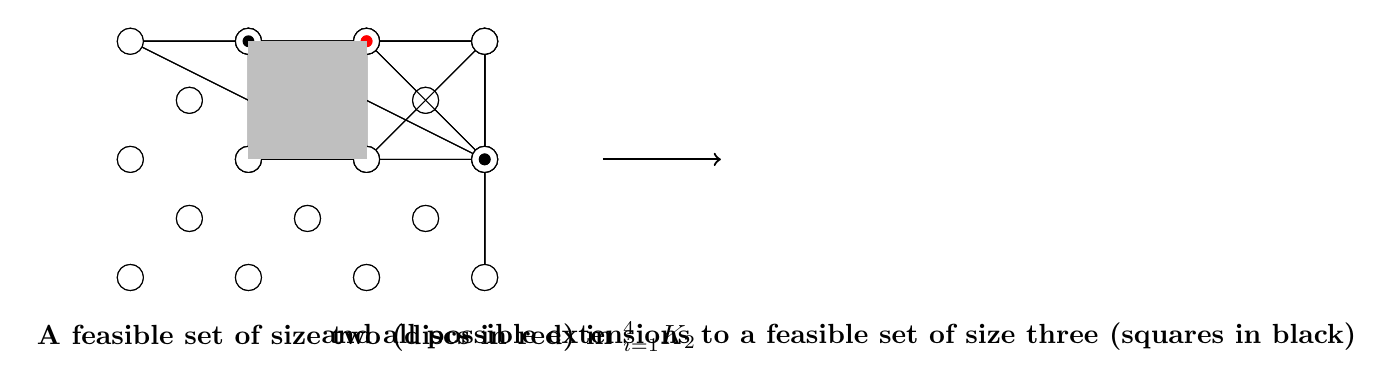
\begin{tikzpicture}[scale=1.5]
    % Define the nodes for the first graph
    \foreach \x in {0,1,2,3} {
        \foreach \y in {0,1,2} {
            \node[circle, draw, fill=white] (n\x\y) at (\x,\y) {};
        }
    }
    \foreach \x in {0,1,2} {
        \foreach \y in {0,1} {
            \node[circle, draw, fill=white] (n\x\y) at (\x+1/2,\y+1/2) {};
        }
    }
    \foreach \x in {0,1,2} {
        \foreach \y in {0,1} {
            \node[circle, draw, fill=white] (n\x\y) at (\x+1,\y+1) {};
        }
    }

    % Draw edges for the first graph
    \draw (n00) -- (n10) -- (n20) -- (n30) -- cycle;
    \draw (n01) -- (n11) -- (n21) -- (n31) -- cycle;
    \draw (n02) -- (n12) -- (n22) -- (n32) -- cycle;
    \draw (n00) -- (n01) -- (n02);
    \draw (n10) -- (n11) -- (n12);
    \draw (n20) -- (n21) -- (n22);
    \draw (n30) -- (n31) -- (n32);
    \draw (n00) -- (n11) -- (n22) -- (n31) -- cycle;
    \draw (n01) -- (n12) -- (n20) -- (n31) -- cycle;
    \draw (n02) -- (n10) -- (n21) -- (n32) -- cycle;

    % Define the nodes for the second graph
    \foreach \x in {0,1,2,3} {
        \foreach \y in {0,1,2} {
            \node[circle, draw, fill=white] (n\x\y) at (\x,\y) {};
        }
    }
    \foreach \x in {0,1,2} {
        \foreach \y in {0,1} {
            \node[circle, draw, fill=white] (n\x\y) at (\x+1/2,\y+1/2) {};
        }
    }
    \foreach \x in {0,1,2} {
        \foreach \y in {0,1} {
            \node[circle, draw, fill=white] (n\x\y) at (\x+1,\y+1) {};
        }
    }

    % Draw edges for the second graph
    \draw (n00) -- (n10) -- (n20) -- (n30) -- cycle;
    \draw (n01) -- (n11) -- (n21) -- (n31) -- cycle;
    \draw (n02) -- (n12) -- (n22) -- (n32) -- cycle;
    \draw (n00) -- (n01) -- (n02);
    \draw (n10) -- (n11) -- (n12);
    \draw (n20) -- (n21) -- (n22);
    \draw (n30) -- (n31) -- (n32);
    \draw (n00) -- (n11) -- (n22) -- (n31) -- cycle;
    \draw (n01) -- (n12) -- (n20) -- (n31) -- cycle;
    \draw (n02) -- (n10) -- (n21) -- (n32) -- cycle;

    % Draw the red discs
    \fill[red] (n11) circle (0.05);
    \fill[red] (n22) circle (0.05);

    % Draw the black squares
    \fill[black] (n31) circle (0.05);
    \fill[black] (n20) circle (0.05);
    \fill[black] (n12) circle (0.05);

    % Draw the gray region
    \fill[gray!50] (n00) rectangle (n22);

    % Draw the arrow
    \draw[->, thick] (4,1) -- (5,1);

    % Label the graphs
    \node at (2,-0.5) {\textbf{A feasible set of size two (discs in red) in $\square_{i=1}^4 K_2$}};
    \node at (6,-0.5) {\textbf{and all possible extensions to a feasible set of size three (squares in black)}};
\end{tikzpicture}

\end{document}